% --------------------------------------------------------------
% This is all preamble stuff that you don't have to worry about.
% Head down to where it says "Start here"
% --------------------------------------------------------------
 
\documentclass[12pt, twoside]{article}
 
\usepackage{fancyhdr}
\usepackage[margin=1in]{geometry} 
\usepackage{amsmath,amsthm,amssymb}

\usepackage{fancyvrb, newverbs}
\usepackage{xcolor}

\usepackage{graphicx}
% -------------------------------------------------------------
% Graphics path
% -------------------------------------------------------------
\graphicspath{{../graphs/}}

% -------------------------------------------------------------
% Verbatim background
% -------------------------------------------------------------
\definecolor{verbbg}{gray}{0.93}
\newverbcommand{\cverb}
  {\setbox\verbbox\hbox\bgroup}
  {\egroup\colorbox{verbbg}{\box\verbbox}}

% -------------------------------------------------------------
% Setup constants 
% -------------------------------------------------------------
\newcommand{\name}{Ethan Febinger, Ryan Mao \\ NetIDs: eef45, rym15}
\newcommand{\class}{CS 440: Intro to AI}
\newcommand{\hwTitle}{Project 1} % Change this for a new homework
\newcommand{\due}{February 19, 2021} % Change this for a new homework


% --------------------------------------------------------------
% Setup header and footer.
% --------------------------------------------------------------
\pagestyle{fancy}
\fancyhf{}
\fancyhead[C]{\hwTitle \hfill \thepage}
\fancyfoot[C]{\name \hfill \class}
\renewcommand{\headrulewidth}{0.4pt} % default is 0pt
\renewcommand{\footrulewidth}{0.4pt} % default is 0pt
 
\newcommand{\N}{\mathbb{N}}
\newcommand{\Z}{\mathbb{Z}}

\newcommand\ddfrac[2]{\frac{\displaystyle #1}{\displaystyle #2}}
 
\newenvironment{theorem}[2][Theorem]{\begin{trivlist}
\item[\hskip \labelsep {\bfseries #1}\hskip \labelsep {\bfseries #2.}]}{\end{trivlist}}
\newenvironment{lemma}[2][Lemma]{\begin{trivlist}
\item[\hskip \labelsep {\bfseries #1}\hskip \labelsep {\bfseries #2.}]}{\end{trivlist}}
\newenvironment{exercise}[2][Exercise]{\begin{trivlist}
\item[\hskip \labelsep {\bfseries #1}\hskip \labelsep {\bfseries #2.}]}{\end{trivlist}}
\newenvironment{problem}[2][Problem]{\begin{trivlist}
\item[\hskip \labelsep {\bfseries #1}\hskip \labelsep {\bfseries #2.}]}{\end{trivlist}}
\newenvironment{question}[2][Question]{\begin{trivlist}
\item[\hskip \labelsep {\bfseries #1}\hskip \labelsep {\bfseries #2.}]}{\end{trivlist}}
\newenvironment{corollary}[2][Corollary]{\begin{trivlist}
\item[\hskip \labelsep {\bfseries #1}\hskip \labelsep {\bfseries #2.}]}{\end{trivlist}}
 
\begin{document}
 
% --------------------------------------------------------------
%                         Start here
% --------------------------------------------------------------
 
\title{\hwTitle} % replace X with the appropriate number
\author{\name\\  % replace with your name
\class} % if necessary, replace with your course title
\date{\due}
 
\maketitle

\section{Integrity}

We, Ryan Mao and Ethan Febinger, certify that the code and report for this assignment are our work alone.

\section{Work Division}
\\
Ryan Mao: Problems 1-4, 6
\\
Ethan Febinger: Problems 5, 7, 8

\section{Preliminaries}
\begin{enumerate}
    \item 
        \textit{Write an algorithm for generating a maze with a given dimension and obstacle density p.}
        
        \vspace{4mm}
        See function \cverb|gen_maze| in \cverb|Maze.py|. \\
        The function takes in two parameters: the first parameter is the desired dimension of the maze, and the second parameter is the desired obstacle density. The maze is represented as a list of lists (a 2D list). The resulting maze will have a $0$ to represent an open square, and a $1$ to represent a square with an obstacle. 

    \item 
        \textit{Write  a  DFS  algorithm  that  takes  a  maze  and  two  locations  within  it,  and             determines whether  one  is  reachable  from  the  other.  Why  is  DFS  a  better  choice  than  BFS  here?  For  as  large  adimension as your system can handle,  generate a plot of ‘obstacle density p’ vs ‘probability that S can be reached from G’.}

        \vspace{4mm}
        See function \cverb|reachable| in \cverb|Maze.py|. \\
        The function uses DFS to determine whether or not there exists a path between the start square and the goal square. The function returns a boolean: \cverb|True| if there exists a path, and similarly, \cverb|False| if you cannot get to the goal from the start. The function does not return any paths.

        \vspace{4mm}
        DFS is a better choice than BFS here since we only wish to determine whether or not the maze is possible to traverse given a start and goal square. Therefore, there is no need to find an optimal path, only a valid path. Due to the nature of the DFS algorithm, it explores as deep as it can before considering branching sideways. In contrast, BFS branches as much as it can before stepping one square deeper. In other words, DFS will go as far as it can until there are no more nodes for it to visit, so it explores nodes farther from the start square (and closer to the goal square), first. If there exists no path, DFS and BFS will take the same amount of time as all squares will be explored regardless.
        % IDK if this makes sense. Maybe add more to this explanation.
        % Since the start and goal squares are constant in this scenario, i.e. start is the top left square and goal is the bottom right square, if we define "deeper" to be to the bottom and to the right, DFS will take on average less time than BFS.
        
        \vspace{4mm}
        For the graph of `obstacle density p' vs `probability that S can be reached from G', we define probability as:
        \begin{center}
            \[\ddfrac{Number\_of\_Successes}{Total\_Sample\_Space}\]
        \end{center}

        Below is a scatter plot generated by the function \cverb|generate_reachable_plot| in \\ \cverb|Graphs.py|.

        \begin{figure}[h]
            \centering
            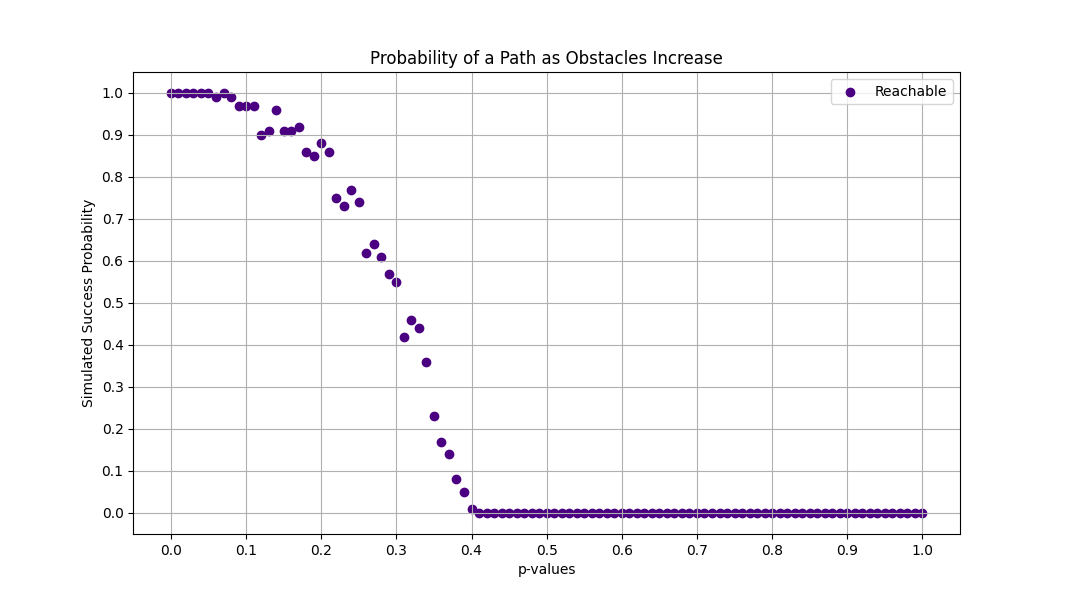
\includegraphics[scale = 0.6]{reachable_scatter.png}
        \end{figure}

        The data for this graph was gathered by generating $100$ mazes at each $p$ value and counting how many of those mazes had a valid path. The mazes were of size $100$. The $p$ values ranged from $0$ to $1$ (inclusive on both sides), with a step of $0.01$. 

        The graph resembles some sort of logistics graph since probability is bounded between $0$ and $1$. The graph is also always decreasing. The slope decreases slowly at first, then begins to decrease faster, but finally flattens out towards the end. 
        
        We see that the probability of a valid path occurring is practically $0$ at a $p$ value of $0.4$ and larger.

        \vfill

    \item
        \textit{Write BFS and A* algorithms (using the euclidean distance metric) that take a maze and determine  the  shortest  path  from S to G if  one  exists.  For  as  large  a  dimension  as  your  system  can handle, generate a plot of the average ‘number of nodes explored by BFS - number of nodes explored by A*’ vs ‘obstacle density p’.  If there is no path from S to G, what should this difference be?}

        \vspace{4mm}
        See function \cverb|BFS| in \cverb|Maze.py|. See function \cverb|AStar| in \cverb|Maze.py|.

        \vspace{4mm}
        For the graph of `number of nodes explored by BFS - number of nodes explored by A*' vs `obstacle density p', we generate a maze using a given dimension and $p$ value, and proceed to run both our BFS and A* algorithms. Both functions return not only a \cverb|True| or \cverb|False| value to represent the existence of a path, but also an optimal path, and the number of squares checked to find said optimal path. Taking the BFS squares explored value, and subtracting the A* squares explored value, gives us the difference in squares explored between the two. Note that this value is always greater or equal to 0 since A* will always explore less than or equal to BFS (In fact, whenever there does NOT exist a valid path, both functions will explore the same amount of squares: i.e. all possible squares reachable from the start square).  

        Below is a scatter plot generated by the function \cverb|generate_BFS_AStar_plot| in \\ \cverb|Graphs.py|.

        \begin{figure}[h]
            \centering
            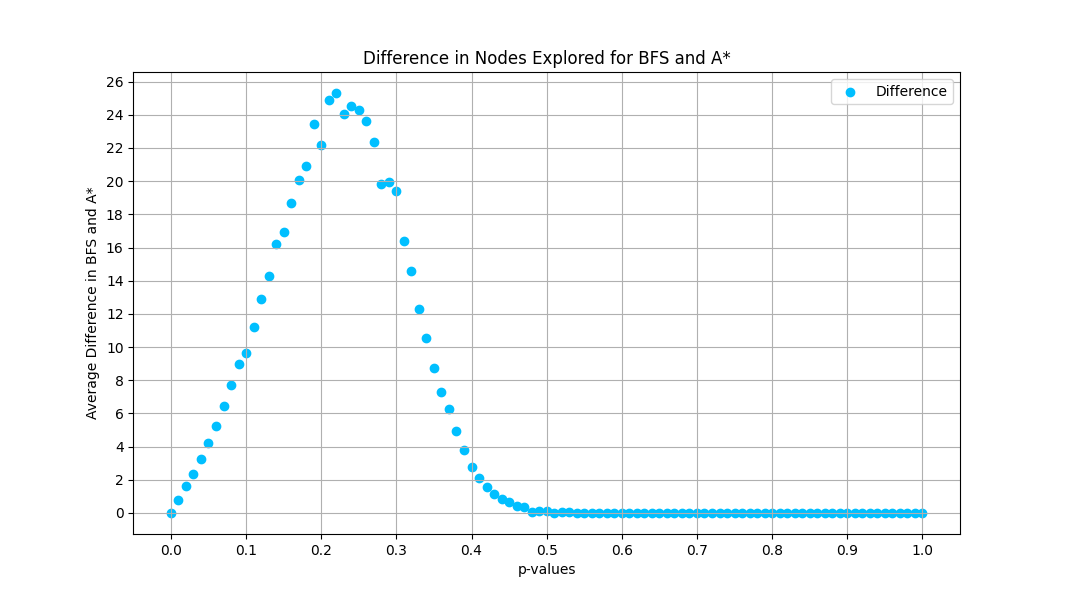
\includegraphics[scale = 0.6]{BFS_AStar_scatter.png}
        \end{figure}

        The data for this graph was gathered by generating $100$ mazes at each $p$ value and summing the difference between the number of squares explored for the two search algorithms. Then we divide the sum by $1,000$ to get the average difference. The mazes were of size $100$. The $p$ values ranged from $0$ to $1$ (inclusive on both sides), with a step of $0.01$.

        \vspace{4mm}
        There seems to be a somewhat linear correlation between $p$ value and the difference in A* vs. BFS from $0$ to $0.3$. Whether the function is actually linear or potentially exponential is unknown. The graph then quickly and drastically falls to $0$ as $p$ approaches $0.4$. This is understandable, as according to our reachable plot in \textbf{Problem 2}, $p$ values close to $0.4$ were practically unreachable. Therefore, A* and BFS would have both been unreachable, and more importantly, both explored the same amount of nodes.
    
    \item
        \textit{What’s the largest dimension you can solve using DFS at p= 0.3 in less than a minute? What’s  the  largest  dimension  you  can  solve  using  BFS  at p= 0.3 in  less  than  a  minute?  What’s  the largest dimension you can solve using A* at p= 0.3 in less than a minute?}

        \vspace{4mm}
        See function \cverb|search_time| in \cverb|Maze.py|. \\
        This function, when given a search algorithm and a maze size, generates mazes until a maze with a valid path is "solved" by the search algorithm (that is a valid/optimal path is found). The return value is the time in seconds that the search algorithm took.

        \vspace{4mm}
        The largest dimension that DFS can solve at a $p$ value of 0.3 in less than a minute (specifically 59 seconds) is $7,500$. The DFS function uses a replicated version of the maze as a visited matrix, allowing us to access and change visited values in constant time. The downside of this, however, is that we must perform a value by value copy, which is inefficient if we only explore a small amount of squares (e.g. if the starting square is surrounded by obstacles, the DFS function still creates the visited matrix).

        \vspace{4mm}
        The largest dimension that BFS can solve at $p$ value of 0.3 in less than a minute (specifically 55 seconds) is $4,550$. However, when we have a maze size of $4,600$, the average compute time is 61 seconds. Therefore, the actual maze size to achieve as close to 60 seconds as possible lies within $4,550$ and $4,600$. These results agree with our predictions, in that BFS takes longer than DFS since it computes for an optimal path rather than simply the existence of one.

        \vspace{4mm}
        The largest dimension that A* can solve at $p$ value of 0.3 in less than a minute (or exactly a minute) is $2,750$. We see from these results that the euclidean distance calculation does in fact add a decent amount of computation time. 

        \vfill

\end{enumerate}
\pagebreak

\section{Given Strategies to Solve the Fire Maze}
\begin{itemize}
    \item[Strategy 1:] 
        \textit{At the start of the maze, wherever the fire is, solve for the shortest path from upper left to lower right, and follow  it  until  the  agent  exits  the  maze  or  burns.   This  strategy  does  not  modify  its  initial  path  as  the  fire changes.}
    
        \vspace{4mm}
        See function \cverb|fire_strategy_1| in \cverb|Maze.py|. \\
        Note that this function does not actually discard mazes that are invalid (by invalid, we mean that there does not exist a path from the start to the goal, there does not exist a path from the start to the starting fire square, or both). \\
        The \cverb|generate_strategy_1_plot| in \cverb|Graphs.py| is actually the function responsible for ensuring that all graphs provided to \cverb|fire_strategy_1| are valid.

        \vspace{4mm}
        Below is a scatter plot generated by the function \cverb|generate_strategy_1_plot| in \cverb|Graphs.py|.

        \begin{figure}[h]
            \centering
            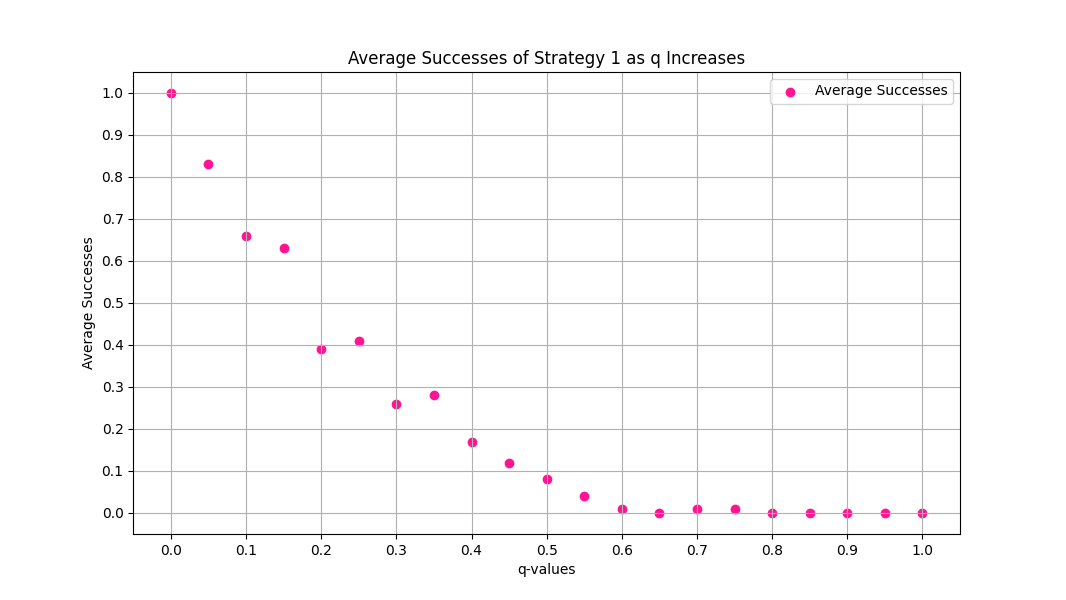
\includegraphics[scale = 0.6]{strategy_1_scatter.png}
        \end{figure}

        Since generating the mazes, and performing the fire spreading, is quite computationally expensive, we could not use as many q-values as we would like. The maze size is $100$, amd each $q$ value has $10$ mazes generated, with each maze then having $10$ different fire starting points.

        \vspace{4mm}
        The graph is always decreasing, and the rate at which it is decreasing is always decreasing. We see that at $0.6$ for $q$, the success rate becomes effectively $0$.

        \pagebreak
    
    \item[Strategy 2:]
        \textit{At every time step, re-compute the shortest path from the agent’s current position to the goal position, based on  the  current  state  of  the  maze  and  the  fire.   Follow  this  new  path  one  time  step,  then  re-compute.   This strategy constantly re-adjusts its plan based on the evolution of the fire.  If the agent gets trapped with no path to the goal, it dies.}

        \vspace{4mm}
        See function \cverb|fire_strategy_2| in \cverb|Maze.py|. \\
        Similarly to \cverb|fire_strategy_1|, this function does not actually discard mazes that are invalid. \\
        The \cverb|generate_strategy_2_plot| in \cverb|Graphs.py| is actually the function responsible for ensuring that all graphs provided to \cverb|fire_strategy_2| are valid.

        \begin{figure}[h]
            \centering
            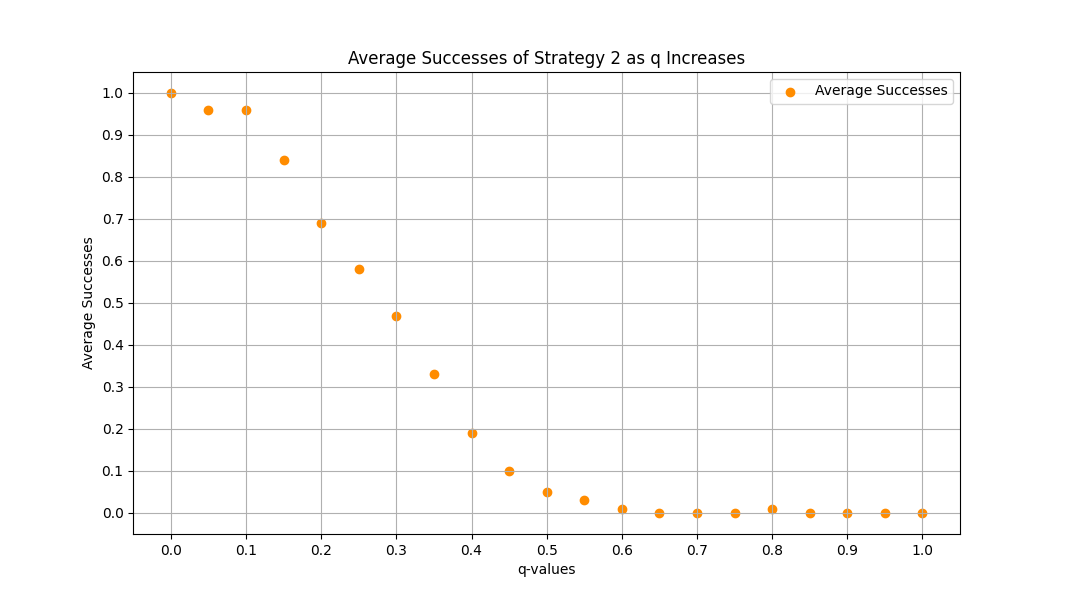
\includegraphics[scale = 0.6]{strategy_2_scatter.png}
        \end{figure}

        The maze size is $100$, amd each $q$ value has $10$ mazes generated, with each maze then having $10$ different fire starting points.

        In comparison to strategy 1, it seems that strategy 2 faired better in the beginning when $q$ was still close to $0$. Both strategy 1 and 2 look to be the same around $0.4$ to $0.5$, with strategy 1 being marginally higher. After $0.6$, both strategies have a practical $0$ average successes.

    \item[Conclusions:]
        \textit{Which strategy performed better?}

        \vspace{4mm}
        Without a doubt, strategy 2 has higher number of average successes than strategy 1. Clearly, adding the extra computations needed to reevaluate and update the path based on new fire spread information helped the survivability of the agent. 


\end{itemize}

\section{Fire Maze}
\begin{enumerate}
    \setcounter{enumi}{4}

    \item \textit{Describe your improved strategy 3. How does it account for the unknown future?}

        \vspace{4mm}
    
    Our strategy 3 accounts for the unknown future by incentivising $A^*$ to find paths that stay away from where the fire is about to spread. Similar to strategy 2, this algorithm recomputes $A^*$ at every timestep to use the most up to date information on where the fire has spread. Instead of having a uniform cost of 1 to travel to any neighboring cell, we increase the cost of traveling to a cell that may be set on fire in the next turn.
    
    \vspace{4mm}
    Our modified $A^*$ function \cverb|AStar_Modified| calls the function \cverb|advance_fire_probability|. This function is sent a copy of the current state of the maze. The maze is stored as a nested list where $0$ represents an empty cell, $1$ represents a barrier cell, and $2$ represents a cell that is on fire. \cverb|advance_fire_probability| iterates through each cell of the maze and changes the value of each empty cell from 0 to the probability it will be set on fire in the next turn. This is calculated by the given formula $1-(1-q)^k$. After this is computed for each cell, the function returns the altered form of the maze.
    
    \vspace{4mm}
    In \cverb|AStar_Modified|, the cost to move to a given cell $(i,j)$ is $1+\alpha *$ maze\_future$[i,j]$ where maze\_future is the modified list obtained from \cverb|advance_fire_probability| and $\alpha$ is a parameter we can adjust to change how aggressively the agent avoids fire. We found $\alpha = 1$ worked best. By increasing the cost, we are discouraging our $A^*$ algorithm from choosing paths that travel nearby the fire. This helps the agent avoid the fire spreading into it while it is traversing the maze, which increases the probability of success.
    
    \item \textit{Plot,  for  Strategy  1,  2,  and  3,  a  graph  of  ‘average  strategy  success  rate’  vs  ‘flammability q’ at p= 0.3.  Where do the different strategies perform the same?  Where do they perform differently?Why?}
    
    \item \textit{If you had unlimited computational resources at your disposal, how could you improve on Strategy 3?}
    
    \vspace{4mm}
    Currently our algorithm accounts for the spread of the fire one timestep into the future. Given unlimited computational resources, we could calculate the probability that a cell will be set on fire for any given timestep in the future. We could then update the cost of traveling to any given cell at any given timestep accordingly. This would allow the agent to look far into the future to avoid areas of the maze where the fire might spread.  
    
    \item \textit{If you could only take ten seconds between moves (rather than doing as much computations as you like), how would that change your strategy?  Describe such a potential Strategy 4.}
    
    
    \vspace{4mm}
    For our current strategy, we are iterating through every point in the maze to determine the probability that the fire will spread to any given cell in the near future. This could be too computationally expensive for a time frame of ten seconds between moves. 
    
    \vspace{4mm}
    A simpler alternative would be to implement a  easy to compute heuristic that would give the agent an idea of how close any given cell is to the fire. This could be achieved by measuring the euclidean distance from a given cell to the starting point of the fire. Then, the cost of moving to any given cell could be increased by a function of this amount. A function such as $f(x)=e^{-x^2}$ would be ideal for this because it increases as $x$ approaches $0$ and goes to $0$ as $x$ approaches infinity. This strategy does not tell the agent of the current location of the fire, but it gives the agent an idea of the general region the fire belongs to and encourages the agent to stay away from this area.

\end{enumerate}
 
% --------------------------------------------------------------
%     You don't have to mess with anything below this line.
% --------------------------------------------------------------
 
\end{document}